\documentclass[a4paper, 11pt]{article}
\usepackage[margin=3cm]{geometry}
\usepackage[utf8]{inputenc}
\usepackage[T1]{fontenc}
\usepackage{amsmath}
\usepackage{amsthm}
\usepackage{tikz}
\usetikzlibrary{arrows, automata}

\newcommand{\code}[1]{\texttt{#1}}

\theoremstyle{definition}
\newtheorem{lemma}{Lemma}

\begin{document}

\author{Lucas Werkmeister}
\title{Ceylon Type System is Chomsky-3 complete}

\maketitle
\tableofcontents

\section{Abstract}

In this article, I will demonstrate an algorithm to transform a finite state automaton into several Ceylon definitions (classes, interfaces, one function), and a second algorithm to transform any word into a Ceylon statement that uses these definitions.
The statement is then well-typed if, and only if, the word is accepted by the automaton.

This proves that the type system / typechecker of the Ceylon programming language is Chomsky-3-complete.

\section{Notation}

\begin{itemize}
\item $\cup$ is the type union operator. $A\cup B$ means the union of types $A$ and $B$ (written \code{A|B} in Ceylon), $\bigcup\limits_{t\in T}t$ means the union of all types in $T$.
\item $\cap$ is the type intersection operator. $A\cap B$ means the intersection of types $A$ and $B$ (written \code{A\&B} in Ceylon), $\bigcap\limits_{t\in T}t$ means the intersection of all types in $T$.
\item $<:$ is the subtype relation. $A<:B$ means that $A$ satisfies $B$ (written \code{A satisfies B} in Ceylon).
\end{itemize}

\section{The automaton}

The automaton is given as a five-tuple $A=(X,Q,q_s,t,F)$, where
\begin{description}
\item[$X$] is the input alphabet $\{x_1,\ldots,x_n\}$,
\item[$Q$] is the set of states $\{q_1,\ldots,q_m\}$,
\item[$q_s$] $\in Q$ is the initial state,
\item[$t$]$: Q\times X\to Q$ is the state transition function, and
\item[$F$] $\subseteq Q$ is the set of accepting states.
\end{description}

We define the auxiliary function $t^\ast: Q\times X\to\{1,\ldots,n\}, (q_i, x_j) \mapsto k: t(q_i, x_j) = q_k$.

\section{The Ceylon definitions}

\begin{itemize}
\item For each character $x_i\in X$ of the input alphabet, define the \code{abstract class X$i$() of x$i$ \{\}} and an \code{object x$i$ extends X$i$() \{\}}.
\item Define the \code{interface Q of $\bigcup\limits_{i=1,\ldots,m}{\code{Q}i}$ \{\}} (so, \code{interface Q of Q1|Q2|\ldots \{\}})
\item For each state $q_i\in Q$, define the \code{interface Q$i$ satisfies Q \{\}}
\item Define the \code{interface B<out T> \{\}} as a box for types
\item Define the \code{alias Accept => B<$\bigcup\limits_{q_i\in F}\code{Q}i$>;}
\item Define the \code{object initial satisfies B<Q$s$> \{\}} (where $q_s$ is the initial state)
\item Define the transition function.
\end{itemize}

\subsection{The transition function}

All the state transitions are encoded into the return type of the transition function \code{t}.
We’ll call that type expression $R$ for now, and look of the rest of the function:

\code{
$R$ t<S,C>(B<S> state, C char)\\
given S of Q\\
given C of $\bigcup\limits_{x_i\in X}\code{X}i$\\
\{return nothing;\}
}

Now comes the last bit.

\[
R = \bigcup\limits_{q_i\in Q}\bigcup\limits_{x_j\in X} \code{S}\cap\code{Q}i \cap \code{C}\cap\code{X}j \cap \code{B<Q}t^\ast(q_i, x_j)\code{>}
\]

\section{The Ceylon expression}

The word $x_{i_1}x_{i_2}\ldots x_{i_k}$ is transformed into the expression
\code{Accept q = t(t(\ldots (t(initial, x$i_1$), x$i_2$), ...), x$i_k$);}

\section{Proof of Chomsky-3-completeness}

I will now attempt to prove that these transformations are correct.

\begin{lemma}\label{disjoint}
The character classes \code{X$i$}, $i=1,\ldots,n$ and the state interfaces \code{Q$i$}, $i=1,\ldots,m$ are disjoint.
\begin{proof}
The declarations of \code{X} and \code{Q} force them to be disjoint.
\end{proof}
\end{lemma}

\begin{lemma}\label{singlestatetransition}
\begin{enumerate}
\item\label{properstatetransition} \[\forall q_k\in Q, x_l\in X: \code{t<Q}k\code{,X}l\code{>} <: \code{B<Q}t^\ast(q_k, x_l)\code{>}\]
In words, the state transition function does exactly what it’s supposed to do.
\item\label{notnothing} \[\forall q_k\in Q, x_l\in X: \code{t<Q}k\code{,X}l\code{>} \neq \code{Nothing}\]
In words, there is always a target state (which can be disjoint from the \code{Accept} type).
\end{enumerate}

\begin{proof}
We recall the return type of the function, with the type arguments filled in:
\[
R = \bigcup\limits_{q_i\in Q}\bigcup\limits_{x_j\in X} \code{Q}k\cap\code{Q}i \cap \code{X}l\cap\code{X}j \cap \code{B<Q}t^\ast(q_i, x_j)\code{>}
\]
From Lemma \ref{disjoint}, we know that the expression $\code{Q}k\cap\code{Q}i$ is \code{Nothing} if $i\neq k$, and that $\code{X}l\cap\code{X}j$ is \code{Nothing} if $j\neq l$. Therefore, the return type can be simplified to:
\begin{align*}
R &= \code{Q}k\cap\code{Q}i \cap \code{X}l\cap\code{X}j \cap \code{B<Q}t^\ast(q_i, x_j)\code{>} \qquad | i=k, j=l\\
  &= \code{Q}k \cap \code{X}l \cap \code{B<Q}t^\ast(q_k, x_l)\code{>}\\
  &<: \code{B<Q}t^\ast(q_k, x_l)\code{>}
\end{align*}
This immediately proves \ref{properstatetransition}. In addition, since of the types $\code{Q}i,\code{X}j,\code{B<Q}k\code{>},i,k=1,\ldots,m,j=1,\ldots,n$ only \code{Q$i$} is a class, these types are not disjoint, and the expression is therefore $\neq \code{Nothing}$, which proves \ref{notnothing}.
\end{proof}
\end{lemma}

\begin{lemma}\label{statetransitions}
\[
x_{i_1}\ldots x_{i_l} \in \mathcal{L}(A) \iff \code{t(\ldots (t(initial, x$i_1$), \ldots), x$i_l$)} <: \code{Accept}
\]
\begin{proof}
By definition of a finite state automaton,
\[x_{i_1}\ldots x_{i_l} \in \mathcal{L}(A) \iff t(\ldots (t(q_s, x_{i_1}), \ldots), x_{i_l})\in F.\]
Therefore, we now must prove
\[t(\ldots (t(q_s, x_{i_1}), \ldots), x_{i_l})\in F \iff \code{t(\ldots (t(initial, x$i_1$), \ldots), x$i_l$)} <: \code{Accept}\]
This statement will follow from the (stronger) statement
\[\code{t(\ldots (t(initial, x$i_1$), \ldots), x$i_l$)} <: \code{B<Q}t^\ast(\ldots (t(q_s, x_{i_1}), \ldots), x_{i_l})\code{>}\]
(“the state always matches”), which we will prove by induction.
\begin{description}
\item[Basis] $l=1$. $\code{t(initial, x}i_1\code{)} <: \code{B<Q}t^\ast(q_s, x_{i_1})\code{>}$ by definition of \code{initial} and Lemma \ref{singlestatetransition}.\ref{properstatetransition}.
\item[Inductive step]
Given that 
\[\code{t(\ldots (t(initial, x}i_1\code{), \ldots), x}i_{l-1}\code{)} <: \code{B<Q}t^\ast(\ldots (t(q_s, x_{i_1}), \ldots), x_{i_{l-1}})\code{>}\]
for some $l$, it follows from Lemma \ref{singlestatetransition}.\ref{properstatetransition} that
\[\code{t(t(\ldots (t(initial, x$i_1$), \ldots), x$i_{l-1}$), x$i_l$)} <: \code{B<Q}t^\ast(t(\ldots (t(q_s, x_{i_1}), \ldots), x_{i_{l-1}}), x_{i_l})\code{>}\]
$\forall x_{i_l} \in X$.
\end{description}
Finally, it follows from the definition of \code{Accept} that
\[\code{B<Q}t^\ast(\ldots(t(q_s, x_{i_1}), \ldots), x_{i_l})\code{>}<:\code{Accept} \iff t(\ldots(t(q_s, x_{i_1}), \ldots), x_{i_l}) \in F\]
\end{proof}
I suck at proofs between code and maths. (Not surprisingly, since this was my first attempt of one.)

If you want to improve it, feel free to submit a pull request!
\end{lemma}

\section{Example}
The following example shows the resulting program for the language accepted by the automaton below (alternatively, it might be expressed through the regular expression $x_1^\ast x_2 x_2^\ast$) and the input word $x_1x_1x_2x_2x_2$.

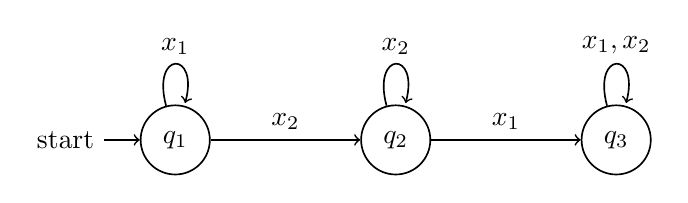
\begin{tikzpicture}[->,auto,node distance=2.8cm,semithick]

\node [initial, state]       (q1) {$q_1$};
\node [state, right of = q1] (q2) {$q_2$};
\node [state, right of = q2] (q3) {$q_3$};

\path (q1) edge [loop above] node {$x_1$} (q1)
           edge              node {$x_2$} (q2)
      (q2) edge              node {$x_1$} (q3)
           edge [loop above] node {$x_2$} (q2)
      (q3) edge [loop above] node {$x_1, x_2$} (q3);

\end{tikzpicture}

\begin{verbatim}
/* alphabet */
abstract class X1() of x1 {} object x1 extends X1() {}
abstract class X2() of x2 {} object x2 extends X2() {}

/* states */
interface Q of Q1|Q2|Q3 {}
interface Q1 satisfies Q {}
interface Q2 satisfies Q {}
interface Q3 satisfies Q {}

"Box around a type"
interface B<out T> {}

"Accepting state(s)"
alias Accept => B<Q2>;

"Initial state"
object initial satisfies B<Q1> {}

"State transition function"
S&Q1&C&X1&B<Q1> |
S&Q1&C&X2&B<Q2> |
S&Q2&C&X1&B<Q3> |
S&Q2&C&X2&B<Q2> |
S&Q3&C&X1&B<Q3> |
S&Q3&C&X2&B<Q3>
        t<S,C>(B<S> state, C x)
        given S of Q
        given C of X1|X2
{ return nothing; }

shared void run() {
    // This statement is well-typed if, and only if, the word composed of the characters in it
    // (read left-to-right) is accepted by the finite state automaton encoded in t.
    Accept q = t(t(t(t(t(initial, x1), x1), x2), x2), x2);
}
\end{verbatim}

\end{document}
